%% LyX 2.2.3 created this file.  For more info, see http://www.lyx.org/.
%% Do not edit unless you really know what you are doing.
\documentclass[english,12pt]{article}
\usepackage{lmodern}
\usepackage[T1]{fontenc}
\usepackage[latin9]{inputenc}
\usepackage{float}
\usepackage{amsmath}
\usepackage{amsthm}
\usepackage{amssymb}
\usepackage{graphicx}

\makeatletter
%%%%%%%%%%%%%%%%%%%%%%%%%%%%%% Textclass specific LaTeX commands.
\theoremstyle{plain}
\newtheorem{thm}{\protect\theoremname}[section]
\theoremstyle{definition}
\newtheorem{defn}[thm]{\protect\definitionname}
\theoremstyle{remark}
\newtheorem{rem}[thm]{\protect\remarkname}
\theoremstyle{definition}
\newtheorem{example}[thm]{\protect\examplename}
\theoremstyle{plain}
\newtheorem{prop}[thm]{\protect\propositionname}
\ifx\proof\undefined
\newenvironment{proof}[1][\protect\proofname]{\par
\normalfont\topsep6\p@\@plus6\p@\relax
\trivlist
\itemindent\parindent
\item[\hskip\labelsep\scshape #1]\ignorespaces
}{%
\endtrivlist\@endpefalse
}
\providecommand{\proofname}{Proof}
\fi
\theoremstyle{definition}
\newtheorem{xca}[thm]{\protect\exercisename}

%%%%%%%%%%%%%%%%%%%%%%%%%%%%%% User specified LaTeX commands.
\usepackage[margin=1in]{geometry}

\makeatother

\usepackage{babel}
\providecommand{\definitionname}{Definition}
\providecommand{\examplename}{Example}
\providecommand{\exercisename}{Exercise}
\providecommand{\propositionname}{Proposition}
\providecommand{\remarkname}{Remark}
\providecommand{\theoremname}{Theorem}

\begin{document}

\title{Math 525: Lecture 4}

\date{January 16, 2018}
\maketitle

\section{Uniform distribution}
\begin{defn}
We say $X$ is \emph{uniformly distributed} on $[a,b]$ (written $X\sim U[a,b]$)
if it is a random variable with distribution function
\[
F(x)=\begin{cases}
0 & \text{if }x<a\\
{\displaystyle \frac{x-a}{b-a}} & \text{if }a\le x<b\\
1 & \text{if }x\geq b.
\end{cases}
\]
\begin{figure}[h]
\begin{centering}
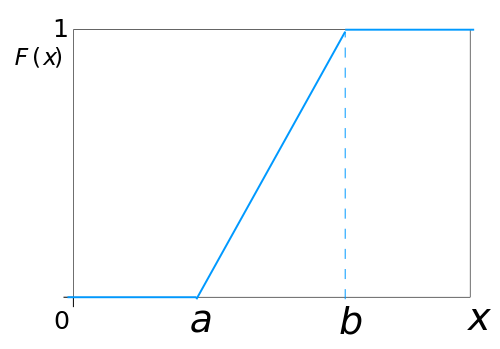
\includegraphics[height=2in]{uniform}
\par\end{centering}
\caption{Uniform distribution}
\end{figure}
\end{defn}
Intuitively, a uniform distribution tells us that any outcome in $[a,b]$
is ``equally likely''.
\begin{rem}
Actually, since $F$ is continuous, no single outcome occurs with
positive probability (recall that $\mathbb{P}(\{X=x\})=F(x)-F(x-)$).
What we really mean is that given two disjoint subsets $A$ and $B$
of $[a,b]$ which have the same ``size'', $X$ is equally likely
to be in either of them.
\end{rem}
\begin{example}
The position of the pointer on a gameshow wheel can be modelled as
a random variable uniformly distributed on $[0,2\pi)$.

\begin{figure}[H]
\begin{centering}

\includegraphics[height=3in]{spinner}
\par\end{centering}
\caption{Game show wheel}
\end{figure}
\end{example}
How do we actually construct a random variable with a uniform distribution?
There are a few ways to do this:
\begin{example}
Let $\Omega=\mathbb{R}$ and $A_{x}=\{\omega\in\Omega\colon\omega\leq x\}$.
Define the probability measure $\mathbb{P}\colon\mathcal{B}(\mathbb{R})\rightarrow[0,1]$
by
\[
\mathbb{P}(A_{x})=\begin{cases}
0 & \text{if }x<a\\
{\displaystyle \frac{x-a}{b-a}} & \text{if }a\le x<b\\
1 & \text{if }x\geq b.
\end{cases}
\]
$(\Omega,\mathcal{B}(\mathbb{R}),\mathbb{P})$ is a probability space.
Moreover, the random variable $X$ defined by $X(\omega)=\omega$
is uniformly distributed on $[a,b]$.
\end{example}
\begin{rem}
You may ask, at this point, why have we not defined $\mathbb{P}$
for sets not of the form $A_{x}$? Remember that $\mathcal{G}=\{A_{x}\}_{x\in\mathbb{R}}$
generates $\mathcal{B}(\mathbb{R})$. It turns out that to define
a probability measure uniquely, it is sufficient to define it on generating
sets (see, e.g., Corollary 1.8 of Walsh, John B. \emph{Knowing the
odds: an introduction to probability}. Vol. 139. American Mathematical
Soc., 2012). The proof of this fact uses something called the \emph{monotone
class theorem}, which is outside of the scope of this course.
\end{rem}
We could have also taken a slightly different approach in defining
a uniformly distributed random variable:
\begin{example}
Let $\Omega=[a,b]$ and $\mathcal{B}([a,b])=\sigma(\{[a,x]\colon x\in\mathbb{R}\})$
(compare this with the definition of $\mathcal{B}(\mathbb{R})$).
Define $A_{x}$ as before and the probability measure $\mathbb{P}\colon\mathcal{B}([a,b])\rightarrow[0,1]$
by
\[
\mathbb{P}(A_{x})=\frac{x-a}{b-a}.
\]
$(\Omega,\mathcal{B}([a,b]),\mathbb{P})$ is a probability space.
Moreover, the random variable $Y$ defined by $Y(\omega)=\omega$
is uniformly distributed on $[a,b]$.
\end{example}
The probability spaces in the last two examples are, for all intents
and purposes, identical... even though $X$ and $Y$ are technically
not the same mathematical objects. The first probability space allows
for points outside of $[a,b]$ to be outcomes, but they occur with
zero probability. The second precludes them altogether.

\section{Existence of random variables}

In the last lecture, we showed that the distribution function $F$
of any random variable is nondecreasing and right-continuous with
\[
\lim_{x\rightarrow-\infty}F(x)=0\qquad\text{and}\qquad\lim_{x\rightarrow\infty}F(x)=1.
\]
Today, we'll prove a ``converse'' of this fact.
\begin{prop}
Let $F\colon\mathbb{R}\rightarrow[0,1]$ be nondecreasing and right-continuous
with 
\[
\lim_{x\rightarrow-\infty}F(x)=0\qquad\text{and}\qquad\lim_{x\rightarrow\infty}F(x)=1.
\]
Then, there exists a random variable whose distribution function is
$F$.
\end{prop}
Note the subtlety here: in the previous lecture, we started out with
a random variable and obtained a distribution function. The above
proposition tells us we can go backwards: start with a distribution
function and obtain a random variable.
\begin{proof}
We only consider the case in which $F$ is a bijection. The general
case is more challenging (see, e.g., Theorem 2.14 of Walsh, John B.
\emph{Knowing the odds: an introduction to probability}. Vol. 139.
American Mathematical Soc., 2012).

Let $X\sim U[0,1]$. In the case that $F$ is a bijection, the inverse
map $F^{-1}$ maps singletons to singletons, and hence can be considered
as a map from $\mathbb{R}$ to $\Omega$. Therefore, we can define
$Y$ by $Y(\omega)=F^{-1}(X(\omega))$, or more succinctly, $Y=F^{-1}\circ X$.
Since $F$ is monotone, so too is $F^{-1}$. As a technical note,
this implies that $F^{-1}$ is Borel measurable and hence $Y$ is
indeed a random variable. Now, note that
\[
\mathbb{P}(\{Y\leq y\})=\mathbb{P}(\{F^{-1}(X)\leq y\})=\mathbb{P}(\{X\leq F(y)\})=\frac{F(y)-0}{1-0}=F(y).\qedhere
\]
\end{proof}
The proof above has a very important consequence for sampling from
non-uniform distributions, as demonstrated below:
\begin{example}
You use a random number generator to generate $n$ samples $U_{1},\ldots,U_{n}\sim U[0,1]$.
You are given the distribution function $F$. Letting $X_{i}=F^{-1}(U_{i})$,
you obtain the samples $X_{1},\ldots,X_{n}$, which all have the distribution
function $F$.
\end{example}
This shows us that we can always turn the problem of sampling from
a non-uniform distribution into one of sampling from a uniform distribution!
\begin{example}
Let $U$ be a uniform random variable on $[0,1]$. Let $X=U^{2}$.
Let $F$ denote the distribution function of $X$. Then, if $0\leq x<1$,
\[
F(x)=\mathbb{P}(\{X\leq x\})=\mathbb{P}(\{U^{2}\leq x\})=\mathbb{P}(\{U\leq\sqrt{x}\})=\sqrt{x}.
\]
\end{example}

\section{Independence of random variables}

In a previous lecture, we defined what it means for two events in
a probability space $(\Omega,\mathcal{F},\mathbb{P})$ to be independent
(if $A,B\in\mathcal{F}$ and $\mathbb{P}(A\cap B)=\mathbb{P}(A)\mathbb{P}(B)$,
we say $A$ and $B$ are independent). We extend this definition now
to random variables.
\begin{defn}
Two random variables $X$ and $Y$ are \emph{independent} if for all
$x,y\in\mathbb{R}$,
\[
\mathbb{P}(\{X\leq x,Y\leq y\})=\mathbb{P}(\{X\leq x\})\mathbb{P}(\{Y\leq y\})
\]
(i.e., the events $\{X\leq x\}$ and $\{X\leq y\}$ are independent).
\end{defn}
\begin{example}
Let $X$ be a random variable. Let $Y=X^{2}$. Suppose $0<\mathbb{P}(\{X\leq a\})<1$
for some $a$. Then,
\[
\mathbb{P}(\{X\leq a,Y\leq a^{2}\})=\mathbb{P}(\{X\leq a,X^{2}\leq a^{2}\})=\mathbb{P}(\{X\leq a,X\leq a\})=\mathbb{P}(\{X\leq a\}).
\]
That is, $X$ and $Y$ are not independent.
\end{example}
The above definition concerns only sets of the form $\{X\leq x\}$
and $\{Y\leq y\}$. Can we extend it to other sets?
\begin{prop}
\label{prop:independence_borel_sets}Let $X$ and $Y$ be independent
random variables. Then,
\[
\mathbb{P}(\{X\in A\}\cap\{Y\in B\})=\mathbb{P}(\{X\in A\})\mathbb{P}(\{Y\in B\})
\]
whenever $A=(p,q]$ and $B=(r,s]$.
\end{prop}
\begin{proof}
Note that
\begin{align*}
\mathbb{P}\{X\in(-\infty,q],Y\in(r,s]\} & =\mathbb{P}\{X\leq q,r<Y\leq s\}\\
 & =\mathbb{P}\{X\leq q,Y\leq s\}-\mathbb{P}\{X\leq q,Y\leq r\}\\
 & =\mathbb{P}\{X\leq q\}\mathbb{P}\{Y\leq s\}-\mathbb{P}\{X\leq q\}\mathbb{P}\{Y\leq r\}\\
 & =\mathbb{P}\{X\leq q\}\left(\mathbb{P}\{Y\leq s\}-\mathbb{P}\{Y\leq r\}\right)\\
 & =\mathbb{P}\{X\leq q\}\mathbb{P}\{r<Y\leq s\}.
\end{align*}
Now, use the same reasoning to get
\[
\mathbb{P}\{p<X\leq q,r<Y\leq s\}=\mathbb{P}\{p<X\leq q\}\mathbb{P}\{r<Y\leq s\}.\qedhere
\]
\end{proof}
\begin{rem}
The previous proposition can be extended more generally to the case
of $A$ and $B$ in $\mathcal{B}(\mathbb{R})$ (see, e.g., Theorem
2.20 of Walsh, John B. \emph{Knowing the odds: an introduction to
probability}. Vol. 139. American Mathematical Soc., 2012). The proof
uses, once again, the monotone class theorem.
\end{rem}

\section{Independence of multiple events}

Let's generalize the concept of independence to families of random
variables.
\begin{defn}
We say the family $\{A_{\alpha}\}_{\alpha\in\mathcal{A}}\in\mathcal{F}$
is independent if for each positive integer $k\leq n$ and $\{A_{i_{1}},\ldots,A_{i_{k}}\}\subset\{A_{\alpha}\}_{\alpha\in\mathcal{A}}$,
\[
\mathbb{P}(A_{i_{1}}\cap\cdots\cap A_{i_{k}})=\mathbb{P}(A_{i_{1}})\cdots\mathbb{P}(A_{i_{k}}).
\]
\end{defn}
The notion of independence above is stronger than requiring each pair
of events to be independent:
\begin{example}
Toss two fair coins at the same time. Let $A$ be the event that the
first coin is heads, $B$ be the event that the second coin is heads,
and $C$ be the event that the first and second coins disagree (i.e.,
one is heads and the other is tails). Note that $\mathbb{P}(A)=\mathbb{P}(B)=\mathbb{P}(C)=1/2$. 

Obviously, $A$ and $B$ are independent. To see that $A$ and $C$
are independent, note that
\[
\mathbb{P}(A\cap C)=1/4=\mathbb{P}(A)\mathbb{P}(C).
\]
Similarly, $B$ and $C$ are independent. This establishes that the
three events are \textbf{pairwise} independent. However, note that
$\mathbb{P}(A\cap B\cap C)=\mathbb{P}(\emptyset)=0$ and $\mathbb{P}(A)\mathbb{P}(B)\mathbb{P}(C)\neq0$.
Therefore, the events $A,B,C$ are not independent, despite being
pairwise independent.
\end{example}
\begin{defn}
We say the family of random variables $\{X_{\alpha}\}_{\alpha\in\mathcal{A}}$
are independent if for each positive integer $k\leq n$, $\{X_{i_{1}},\ldots,X_{i_{k}}\}\subset\{X_{\alpha}\}_{\alpha\in\mathcal{A}}$,
and $x_{1},\ldots,x_{k}$, 
\[
\mathbb{P}(\{X_{i_{1}}\leq x_{1},\ldots,X_{i_{k}}\leq x_{n}\})=\mathbb{P}(\{X_{i_{1}}\leq x_{1}\})\cdots\mathbb{P}(\{X_{i_{k}}\leq x_{n}\}).
\]
\end{defn}
\begin{xca}
Let $X$ and $Y$ be i.i.d. integer-valued random variables (i.e.,
$\mathbb{P}(\{X\text{ is an integer}\})=1$ and similarly for $Y$).
Let $p_{n}=\mathbb{P}(\{X=n\})$. Then,
\[
\mathbb{P}(\{X=Y\})=\sum_{n=-\infty}^{\infty}\mathbb{P}(\{X=n\})\mathbb{P}(\{Y=n\})=\sum_{n=-\infty}^{\infty}p_{n}^{2}.
\]
Similarly,
\[
\mathbb{P}(\{X\leq Y\})=\sum_{n=-\infty}^{\infty}\mathbb{P}(\{X=n\})\sum_{m=n}^{\infty}\mathbb{P}(\{Y=n\})=\sum_{n=-\infty}^{\infty}p_{n}\sum_{m=n}^{\infty}p_{m}.
\]
For example, suppose
\[
p_{n}=\frac{6}{\pi^{2}}\frac{1}{n^{2}}\text{ if }n>0\qquad\text{and}\qquad p_{n}=0\text{ otherwise}
\]
(you can check that $\sum_{n=1}^{\infty}p_{n}=1$). Then,
\[
\mathbb{P}(\{X=Y\})=\sum_{n=1}^{\infty}p_{n}=\frac{36}{\pi^{4}}\sum_{n=1}^{\infty}\frac{1}{n^{4}}=\frac{36}{\pi^{4}}\frac{\pi^{4}}{90}=\frac{36}{90}=\frac{2}{5}.
\]
and
\[
\mathbb{P}(\{X\leq Y\})=\sum_{n=1}^{\infty}p_{n}\sum_{m=n}^{\infty}p_{m}=\frac{36}{\pi^{4}}\sum_{n=1}^{\infty}\frac{1}{n^{2}}\sum_{m=n}^{\infty}\frac{1}{m^{2}}=\frac{36}{\pi^{4}}\frac{7\pi^{4}}{360}=\frac{7}{10}.
\]
\end{xca}

\section{Types of distributions}
\begin{defn}
Let $X$ be a random variable.
\begin{enumerate}
\item $X$ has a \emph{discrete distribution} if we can find a countable
subset $\{x_{n}\}_{n}\subset\mathbb{R}$ for which
\[
\sum_{n=1}^{\infty}\mathbb{P}\{X=x_{n}\}=1.
\]
\item $X$ has a \emph{continuous distribution} if its distribution function
$F$ is continuous.
\item $X$ has an \emph{absolutely continuous distribution} if its distribution
function can be written
\[
F(x)=\int_{-\infty}^{x}f(y)dy
\]
for some integrable function $f$.
\end{enumerate}
\end{defn}
While many random variables fall into one of the above categories,
there are still many which do not! For example...
\begin{example}
Consider flipping a coin. If the coin is heads, you receive one dollar.
Otherwise, you receive $Y$ dollars, where $Y\sim U[0,1]$. This random
variable is
\[
X=I_{\{\text{tails}\}}Y+I_{\{\text{heads}\}}.
\]
Its distribution function is
\[
F(x)=\begin{cases}
0 & \text{if }x<0\\
{\displaystyle \frac{x}{2}} & \text{if }0\leq x<1\\
1 & \text{if }x\geq1.
\end{cases}
\]
\end{example}

\end{document}
